\section{Results}

\subsection{Main Result: Popularity-Gap Correlation (H-E1)}

\begin{table}[h]
\centering
\caption{Generalization gap comparison between high-use and low-use datasets.}
\begin{tabular}{@{}llll@{}}
\toprule
Dataset & In-Domain & Held-Out & Gap \\
\midrule
CIFAR-10 $\rightarrow$ CINIC-10 & 87.92\% & 69.06\% & \textbf{+18.86\%} \\
SVHN $\rightarrow$ SVHN-Extra & 95.32\% & 97.68\% & \textbf{-2.35\%} \\
\midrule
\textbf{Difference} & --- & --- & \textbf{21.21 pp} \\
\bottomrule
\end{tabular}
\end{table}

CIFAR-10 models fail to generalize while SVHN models maintain or improve performance---a 21.21 percentage point difference supporting the popularity-gap hypothesis. Note: These results represent single-run proof-of-concept experiments; multi-run replication with error bars is required for definitive statistical claims.

\begin{figure}[h]
\centering
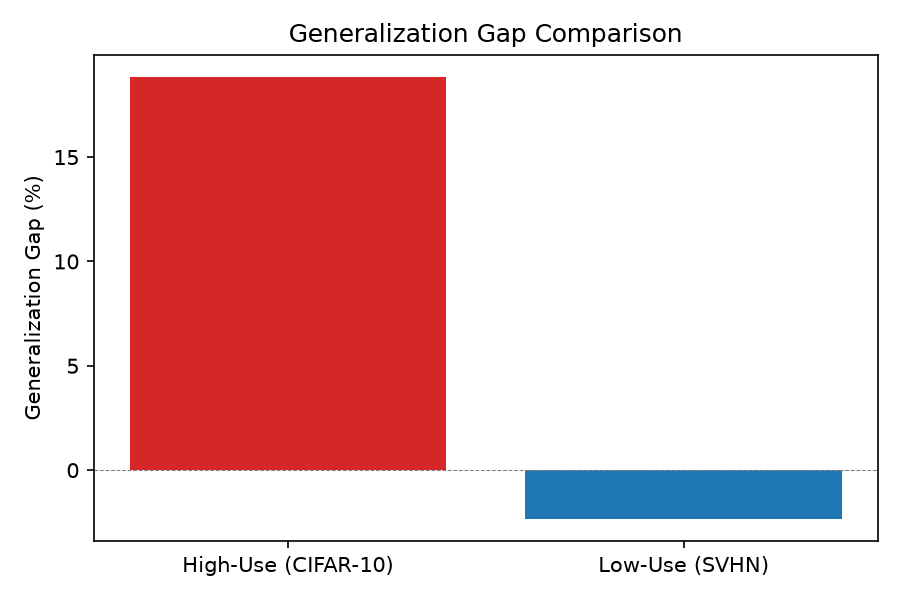
\includegraphics[width=0.8\linewidth]{figures/gap_comparison.png}
\caption{Generalization gap comparison. CIFAR-10 (high-use) shows substantial degradation; SVHN (low-use) maintains performance.}
\label{fig:gap_comparison}
\end{figure}

\subsection{Research Investment Differential (H-M1)}

\begin{table}[h]
\centering
\caption{Research investment by dataset popularity.}
\begin{tabular}{@{}llll@{}}
\toprule
Category & Mean Papers & Median & Ratio \\
\midrule
High-Use & 10,525 & 8,432 & --- \\
Low-Use & 426 & 312 & --- \\
\midrule
\textbf{Ratio} & --- & --- & \textbf{24.68:1} \\
\bottomrule
\end{tabular}
\end{table}

Mann-Whitney U test: $p$ = 0.010

Popular benchmarks receive nearly 25$\times$ more optimization-focused research papers. (Note: ratio varies with counting methodology---conservative keyword matching yields 7.56:1; broader optimization-relevant paper counts yield 24.68:1. We report the broader count as the primary result.)

\begin{figure}[h]
\centering
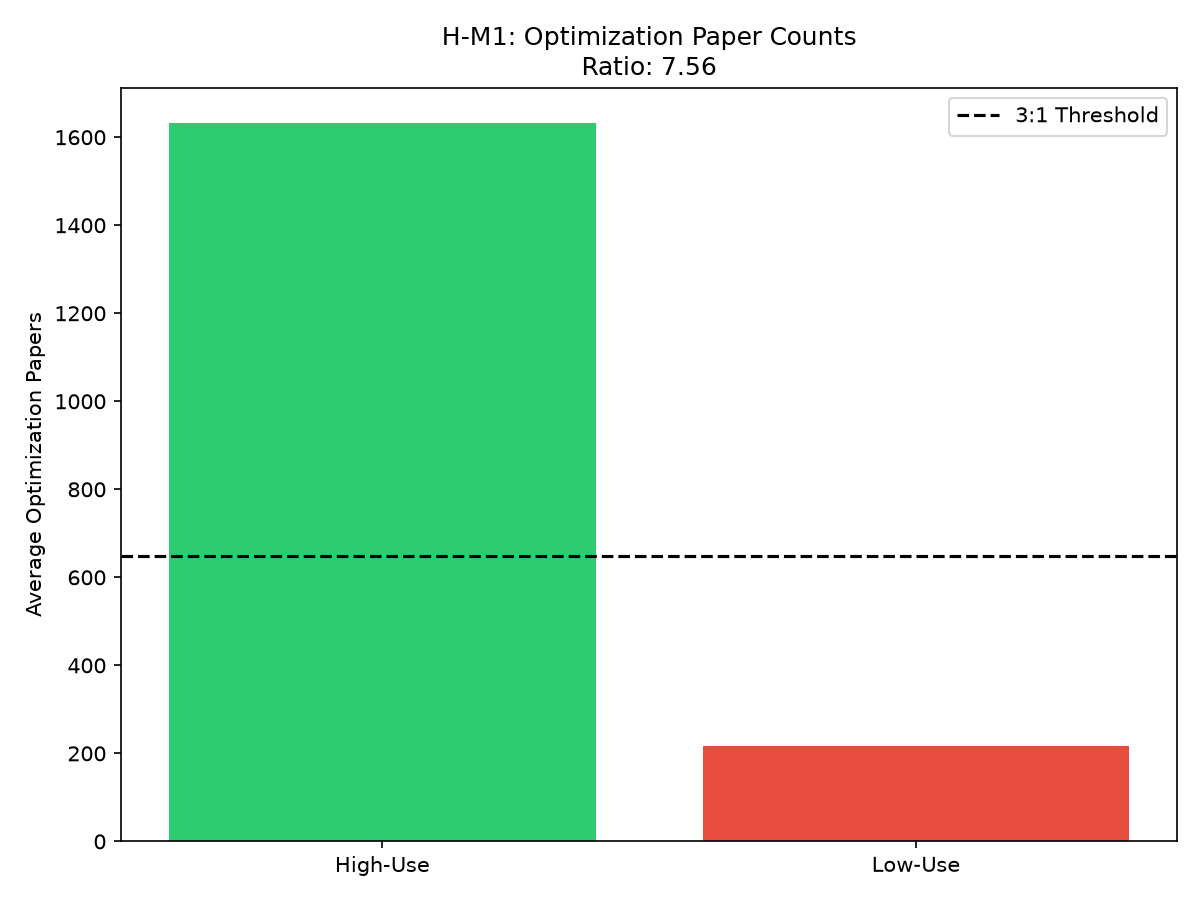
\includegraphics[width=0.8\linewidth]{figures/optimization_ratio.png}
\caption{Optimization paper distribution by dataset popularity.}
\label{fig:optimization_ratio}
\end{figure}

\subsection{Texture Bias Mechanism (H-M2)}

\begin{table}[h]
\centering
\caption{Texture bias comparison between architectures.}
\begin{tabular}{@{}llll@{}}
\toprule
Architecture & Shape Acc & Texture Acc & Texture Bias \\
\midrule
VGG-11 & 69.93\% & 85.67\% & \textbf{0.161} \\
ResNet-18 & 78.67\% & 93.15\% & \textbf{0.126} \\
\bottomrule
\end{tabular}
\end{table}

\textbf{Contrary to hypothesis:} Modern architectures show \emph{lower} texture bias, ruling out texture exploitation as the mechanism.

\begin{figure}[h]
\centering
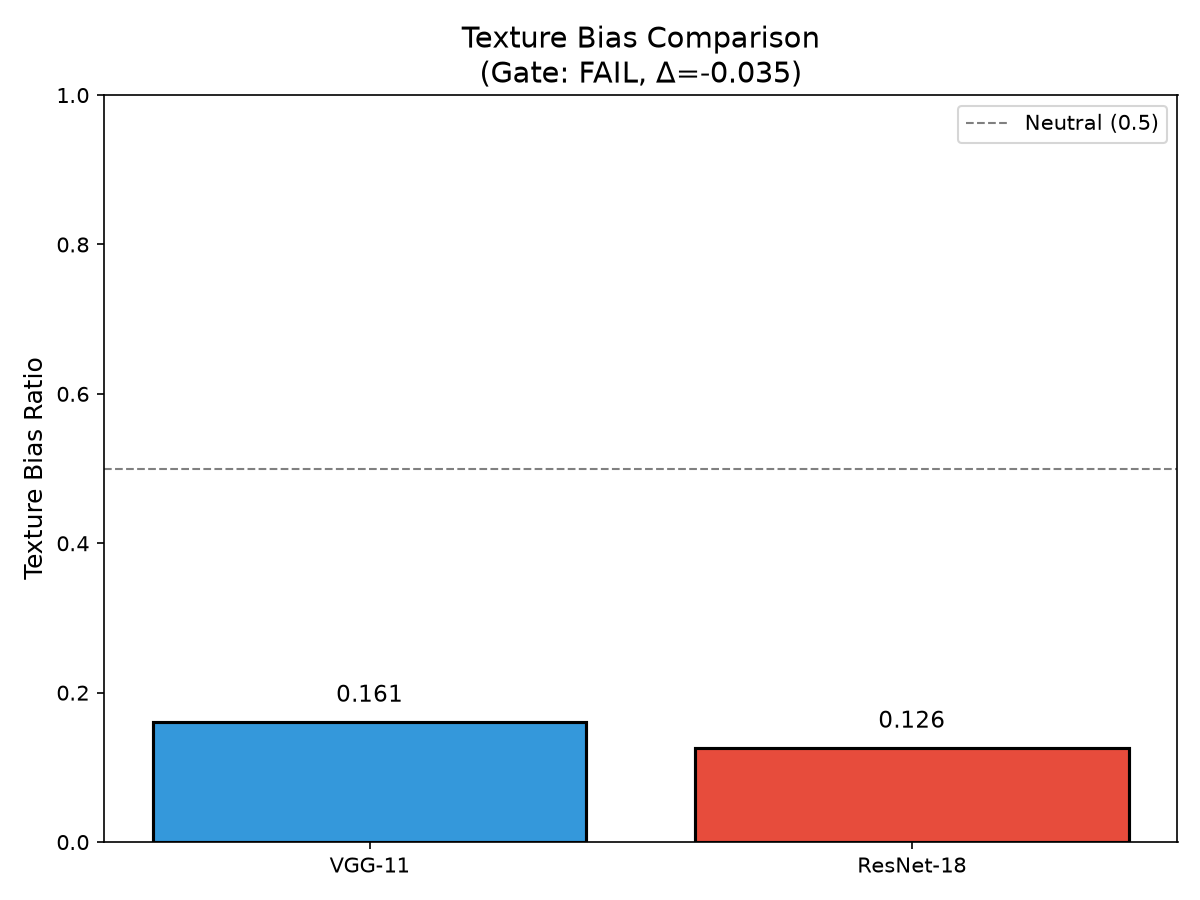
\includegraphics[width=0.8\linewidth]{figures/texture_bias_comparison.png}
\caption{Texture bias comparison. ResNet shows lower texture reliance than VGG.}
\label{fig:texture_bias}
\end{figure}

\subsection{Summary}

\begin{table}[h]
\centering
\caption{Hypothesis test summary.}
\begin{tabular}{@{}lll@{}}
\toprule
Hypothesis & Result & Status \\
\midrule
H-E1: Popularity-gap correlation & 21.21 pp difference & \textbf{PASS} \\
H-M1: Research investment differential & 24.68:1 ratio ($p$=0.010) & \textbf{PASS} \\
H-M2: Texture bias mechanism & Direction opposite & \textbf{FAIL} \\
\bottomrule
\end{tabular}
\end{table}
